
\begin{subsection}{Diagrama de contexto}
En la figura \ref{fig:diagrama_contexto} puede verse el diagrama de contexto el cual, captura todos los agentes y fenómenos relativos al sistema anteriormente descripto.

\begin{figure}[!ht]
\begin{center}
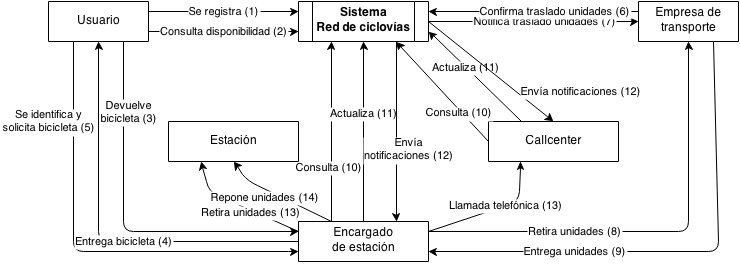
\includegraphics[scale=0.60]{imagenes/diagrama_contexto.png}
\caption{diagrama de contexto}
\label{fig:diagrama_contexto}
\end{center}
\end{figure}
\end{subsection}

\begin{subsection}{Agentes}
	\begin{itemize}
	\item Persona.
	\item Usuario.
	\item Encargado de terminal.
	\item Callcenter.
	\item Gobierno.
	\item Agencia de Estadística.
	\item Empresa de transporte.
	\end{itemize}
\end{subsection}

\begin{subsection}{Eventos}

%\textit{(Formato: Nro. de evento- Evento. \{Nro. de interacción entre agentes en el diagrama\})}

%	\begin{itemize}
%	\item [1-] EL USUARIO se registra por internet con el SISTEMA. \{\textbf{1}\}
%	\end{itemize} 
	
	\begin{enumerate}
	\item Ingresa datos por web.
	\item Informa registración exitosa.
	\item Ingresa datos por terminal en estación.
	\item Brinda datos por teléfono.
	\item Ingresa datos brindados.
	\item Informa registración exitosa.
	\item Informa registración exitosa.
	\item Presenta documentación.
	\item Verifica datos de usuario.
	\item Confirma validación de usuario.
	\item Confirma validación.
	\item Confirma datos por teléfono.
	\item Confirma datos.
	\item Confirma validación.
	\item Confirma validación.
	\item Genera problema de registración.
	\item Confirma registración de problema.
	\item Consulta usuarios con problemas de registración.
	\item Remueve usuario con problemas de registración.
	\item Confirma remoción de usuario.
	\item Solicita stock de estación vía web.
	\item Informa stock de estación.
	\item Consulta datos recolectados.
	\item Confirma o modifica el umbral.
	\item Envía pedido de reposición.
	\item Notifica recepción de pedido.
	\item Envía pedido de reposición.
	\item Notifica pedido de reposición.
	\item Notifica recepción del pedido.
	\item Notifica recepción del pedido.
	\item Actualiza cantidad de bicicletas entregadas/recibidas.
	\item Informa actualización de stock.
	\item Actualiza cantidad de bicicletas entregadas/recibidas por teléfono.
	\item Actualiza cantidad de bicicletas entregadas/recibidas.
	\item Informa actualización de stock.
	\item Informa actualización de stock exitosa.
	\item Identifica usuario.
	\item Confirma identificación.
	\item Confirma identificación.
	\item Identificar usuario por teléfono.
	\item Identificar usuario.
	\item Confirma identifiación.
	\item Confirma identifiación.
	\item Consulta penalizaciones.
	\item Informa penalizaciones pendientes.
	\item Consulta penalizaciones por teléfono.
	\item Consulta penalizaciones.
	\item Informa penalizaciones pendientes.
	\item Informa penalizaciones pendientes.
	\item Informa penalizaciones pendientes.
	\item Consulta usuarios penalizados.
	\item Remueve usuarios penalizados.
	\item Confirmar remoción del usuario.
	\item Almacena datos de uso y funcionamiento.
	\item Consulta datos de uso y funcionamiento.
	\item Actualiza estado de usuario.
	\item Informa estado del usuario.
	\end{enumerate}

\end{subsection}